\documentclass[12pt,a4paper,oneside,openany]{memoir}

\usepackage[utf8]{inputenc}
\usepackage[frenchb]{babel}
\usepackage[T1]{fontenc}


% Paquets utiles
\usepackage{graphicx}
\usepackage[usenames,svgnames]{xcolor}
\usepackage{tikz}
\usepackage{asymptote}
\usepackage{flafter}
\usepackage{multirow}
\usepackage{ifdraft}
\usepackage{units}
\usepackage{booktabs}
%\usepackage[pdfpagelabels,draft,implicit=false]{hyperref}

%Tkiz
\usetikzlibrary{calc}
\usetikzlibrary{arrows}


% Décoration
\usepackage[lighttt]{lmodern} % pour le tt


% POUR MATHDESIGN : restaurer hrulefill
\let\xhrf\hrulefill
\usepackage[utopia]{mathdesign}
\let\hrulefill\xhrf
\renewcommand*{\chapterheadstart}{\begingroup
	\vspace*{\beforechapskip}%
	\begin{adjustwidth}{}{-\chapindent}%
		\hrulefill
		\smash{\rule{0.4pt}{15mm}}
	\end{adjustwidth}\endgroup}
%\usepackage{tgpagella}
\let\mathbb\relax \usepackage{bbold}
\fixpdflayout
%\counterwithout{section}{chapter}
%\setsecnumdepth{subsection}


\chapterstyle{ell}
\setsecheadstyle{\Large\bfseries\sffamily\raggedright}
\setsubsecheadstyle{\large\bfseries\sffamily\raggedright}
\midsloppy

\makepagestyle{myruled}
\makeoddfoot{myruled}{}{\thepage}{}
\makeevenfoot{myruled}{}{\thepage}{}
\makeheadrule{myruled}{\textwidth}{\normalrulethickness}
\makeevenhead{myruled}{\rightmark}{}{}
\makeoddhead{myruled}{\rightmark}{}{}
\pagestyle{myruled}

\captiondelim{ : }
\captiontitlefont{\sffamily}

\newsubfloat{figure}
\newsubfloat{table}

\newcommand{\anonchapter}[1]{\chapter*{#1}\addcontentsline{toc}{chapter}{\numberline{}#1}}
\newcommand{\todo}[1]{\marginpar{\textcolor{red}{#1}}}
\newcommand{\fltbrule}{\hrule\vspace{\onelineskip}}
\newcommand{\fltarule}{\vspace{\onelineskip}
	\hrule\vspace{\onelineskip}}

\author{Charles Bine\\Matthieu Félix}
\title{\\Production d'énergie électrique (centrales nucléaires et barrages hydroélectriques)}
\date{Décembre 2015}


% EXEMPLES & référence rapide
% dessin asymptote
% \lstinputlisting[firstline=, lastline=]{fichier}

\begin{document}
	
% Page de titre
\keepthetitle
\begin{titlingpage}
\noindent
\begin{minipage}[t]{0.4\textwidth} \begin{flushleft}
\theauthor \\ \thedate
\end{flushleft} \end{minipage}
\begin{minipage}[t]{0.4\textwidth} \begin{flushright}
Rapport de projet
Cours de réseaux électriques
\end{flushright} \end{minipage}

\vspace{3cm}
\begin{center}
{\LARGE \textsc{\thetitle}}
\ifdraft{\par Brouillon}{}
\end{center}
\vspace{3cm}

\end{titlingpage}

\addtolength{\marginparwidth}{11mm}
\abnormalparskip{4mm}

\clearpage

\tableofcontents
\listoffigures
\listoftables
\clearpage


\chapter{Introduction}

Dans le sillage de la mondialisation, les enjeux de la production et de la consommation énergétiques sont capitaux. La demande énergétique mondiale, toujours croissante, requiert l'inauguration d'un nombre toujours plus important de centrales de production d'énergie.

Mais comment produire durablement cette énergie? Quelles méthodes choisir? Comment respecter aux mieux les recommandation établies lord de la COP 21 à Paris? 


\chapter{Aperçu de la production d'énergie électrique}

Les principales ressources énergétiques sont les énergies fossiles (le gaz naturel, le charbon, le pétrole), l’énergie hydroélectrique, l’énergie éolienne, l’énergie nucléaire, l’énergie solaire et l'énergie géothermique. 

Étant donné les impacts environnementaux des énergies fossiles, nous nous attarderons dans cet article à l'analyse de deux types de production d'énergie électrique renouvelable: les centrales nucléaires et les barrages hydroélectriques. 

\section{Production mondiale}

L'électricité est communément présentée comme une "énergie propre". En effet les équipements l'utilisant n'émettent aucun gaz polluant ni gaz à effet de serre directement du fait de l'utilisation de l'énergie électrique.
Toutefois l'électricité n'est pas une énergie disponible naturellement sur Terre ; elle est donc produite par conversion d'autres formes d'énergie en énergie électrique.
Or la plupart des processus de production d'électricité, et en particulier ceux les plus répandus au début du XX\ieme{} siècle, ont des effets néfastes sur l'environnement :


\paragraph{Les centrales thermiques} rejettent des oxydes de soufre, d'azote et des suies et surtout émettent d'importantes quantités de CO2 (principal gaz à effet de serre) ;
\paragraph{Les centrales nucléaires} produisent des déchets radioactifs dont la durée de vie peut dépasser le millénaire ;
\paragraph{Les grands barrages hydroélectriques}  modifient profondément les écosystèmes (Voir Barrage des Trois-Gorges en Chine);
\paragraph{Les éoliennes} défigureraient, aux yeux de certains, les paysages.


L'électricité, comme toutes les formes ou vecteurs énergétiques, génère donc des impacts environnementaux, économiques et sociaux que l'on cherche à limiter. Toutefois, la répartition des formes d'énergie laisse toujours à désirer. En effet, les figures \ref{fig:monde1} et \ref{fig:monde2} montrent la prédominance des énergies fossiles dans le monde.

\begin{figure}[h]
	\centering]\hspace*{-5mm}
	\begin{minipage}{.5\textwidth}
		\centering
		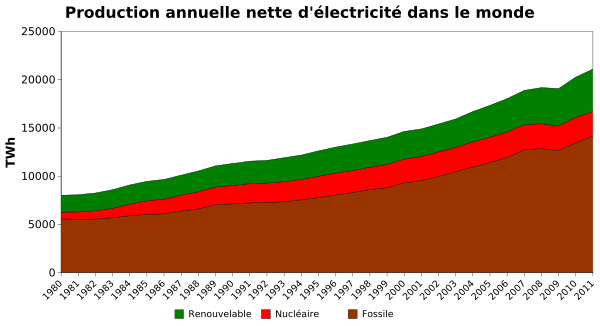
\includegraphics[width=\linewidth]{img/monde1.png}
		\caption{Évolution de la répartition de la production d'énergie mondiale}
		\label{fig:monde1}
	\end{minipage}%
	\hspace*{1cm}
	\begin{minipage}{.5\textwidth}
		\centering
		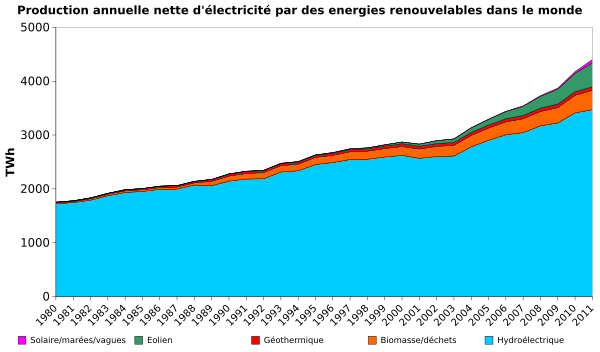
\includegraphics[width=\linewidth]{img/monde2.png}
		\caption{Évolution de la répartition de la production d'énergie renouvelable mondiale}
		\label{fig:monde2}
	\end{minipage}
\end{figure}



\section{Production Française}

Après la disparition complète de la production française de charbon en 2005, le pétrole, le gaz et surtout l’électricité sont les principales énergies consommées en France. Si la France ne produit plus de pétrole brut que de façon marginale, les treize raffineries implantées sur le territoire permettent de satisfaire plus de 90 \% de la demande nationale. Le groupe français Total, qui possède des concessions dans le monde entier, est la sixième entreprise mondiale et la cinquième du secteur. La part du gaz dans la consommation énergétique française a fortement augmenté depuis les années 1970, mais il s’agit à 97 \% de gaz importé, notamment de Russie, d’Algérie et de la mer du Nord. 

En revanche, la France produit plus d’électricité qu’elle n’en consomme, notamment grâce à 59 réacteurs nucléaires (le second parc mondial après le parc américain) qui produisaient en 2013 près de 74\% de l’électricité du pays, mais dont le bilan environnemental est l’objet de débats. Quant aux énergies renouvelables, leur part dans la production électrique française augmente et s’établit en 2013 à près de 17 \%, en grande partie grâce à l’hydroélectrique. 

Le tableau \ref{repartition production} détaille les différents composants de la production énergétique française en fonction du type de production d'énergie.

	\begin{table}[h]
		\centering
		\begin{tabular}{cc}
			\toprule
			Filière & Répartition\\
			\midrule
			Nucléaire & $74\%$ \\ 
			Hydro & $13,3\%$ \\ 
			Thermique & $7,8\%$ \\ 
			Éoliennes & $2,8\%$ \\ 
			Autres & $0,9\%$ \\ 
			Biomasse & $0,7\%$ \\ 
			\bottomrule
		\end{tabular} 
		\caption{Répartition de la production énergétique par filière}
		\label{repartition production}
	\end{table}


La consommation française d'électricité s'élève à environ \unit[480]{TWh} par an. Cependant, la consommation est assujettie à des fluctuations parfois importantes, souvent dues à des contingences météorologiques. 

\begin{figure}[h]
	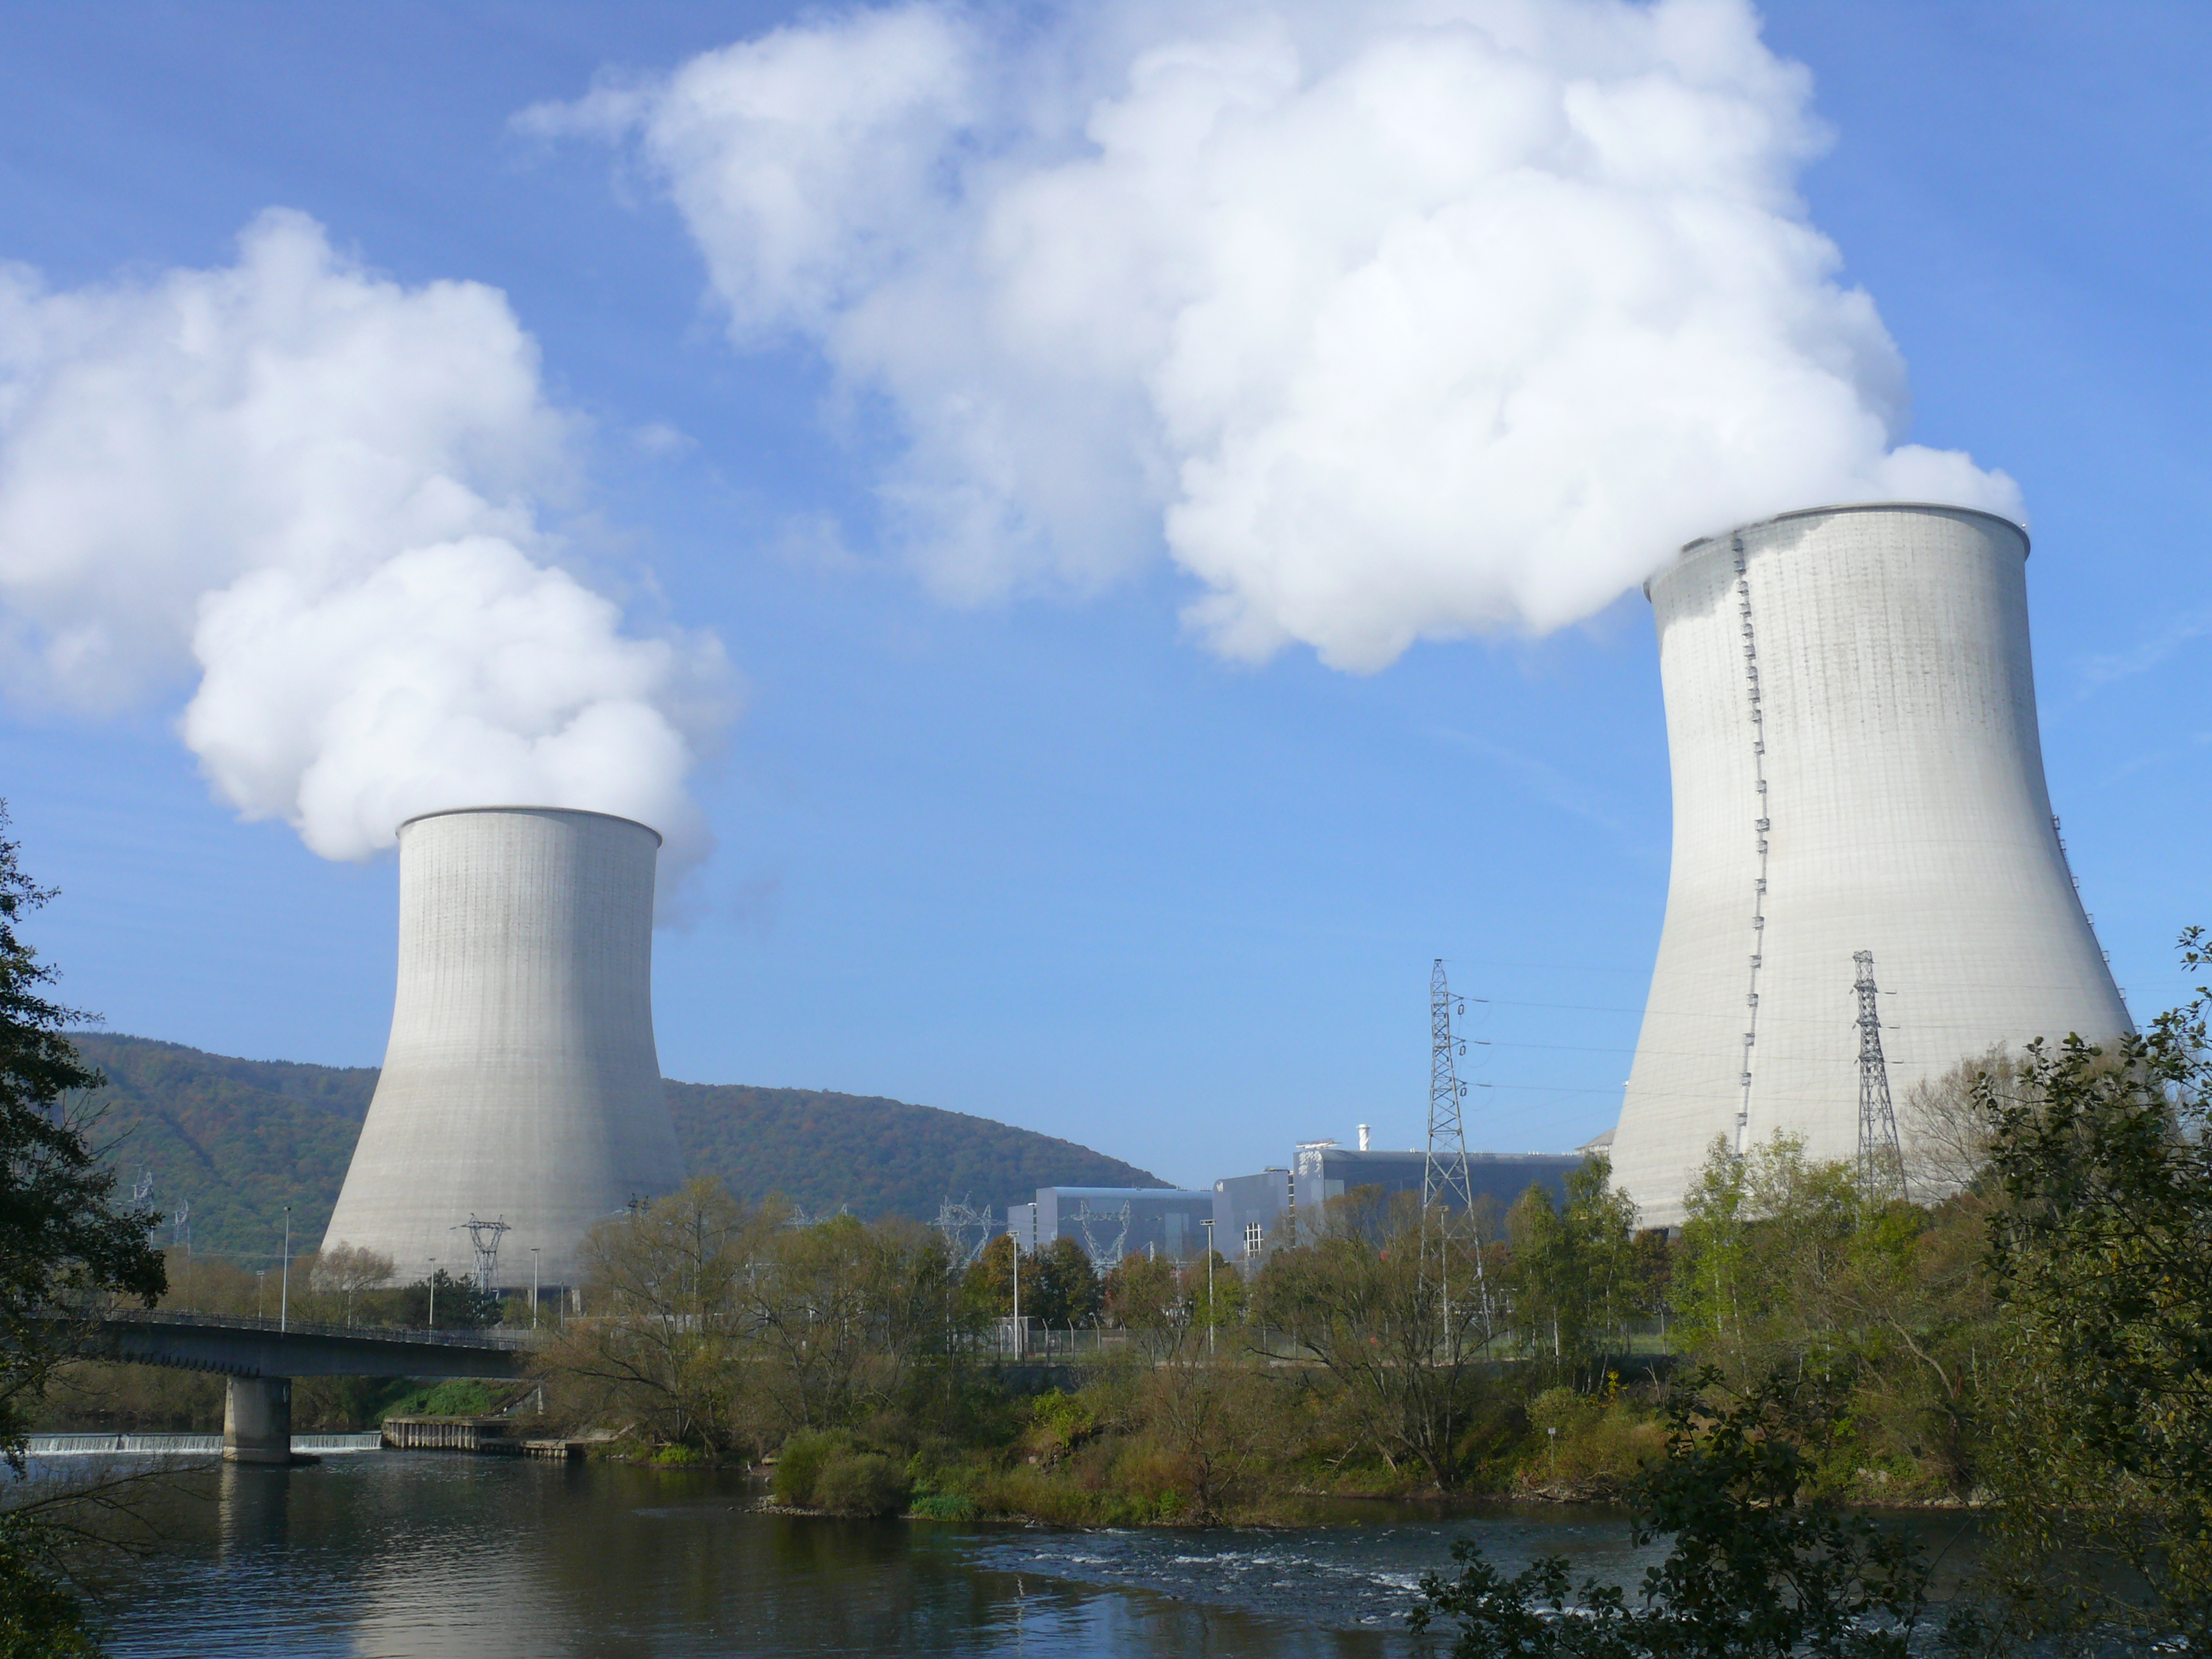
\includegraphics[width=\textwidth]{img/centrale1.jpeg}
	\caption[Une photographie de la Centrale nucléaire de Chooz]{Une photographie de la Centrale nucléaire de Chooz, construite et opérée par EDF.}
\end{figure}

La répartition de la consommation de l'électricité par secteur est représentée dans la table \ref{repartition secteur}. On constate que les deux tiers de la consommation française sont dus aux ménages et aux transports.



	\begin{table}[h]
		\centering
		\begin{tabular}{cc}
			\toprule
			Secteur & Répartition\\
			\midrule
			Ménages & $30,3\%$ \\ 
			Industrie & $19,4\%$ \\ 
			Transports & $31,1\%$ \\ 
			Services & $16\%$ \\ 
			Agriculture & $3\%$ \\ 
			Pèche & $0,2\%$ \\ 
			\bottomrule
		\end{tabular} 
		\caption{Répartition de la consommation énergétique par secteur}
		\label{repartition secteur}
	\end{table}













\chapter{L'alternateur, au cœur de la production d'énergie électrique}

\chapter{La centrale nucléaire}




\chapter{Le barrage hydroélectrique}

\end{document}
